% 4章
\chapter{統合試験}
\label{chap:test}

%********************************
%図の追加
%\begin{figure}[H]
%	\centering
%	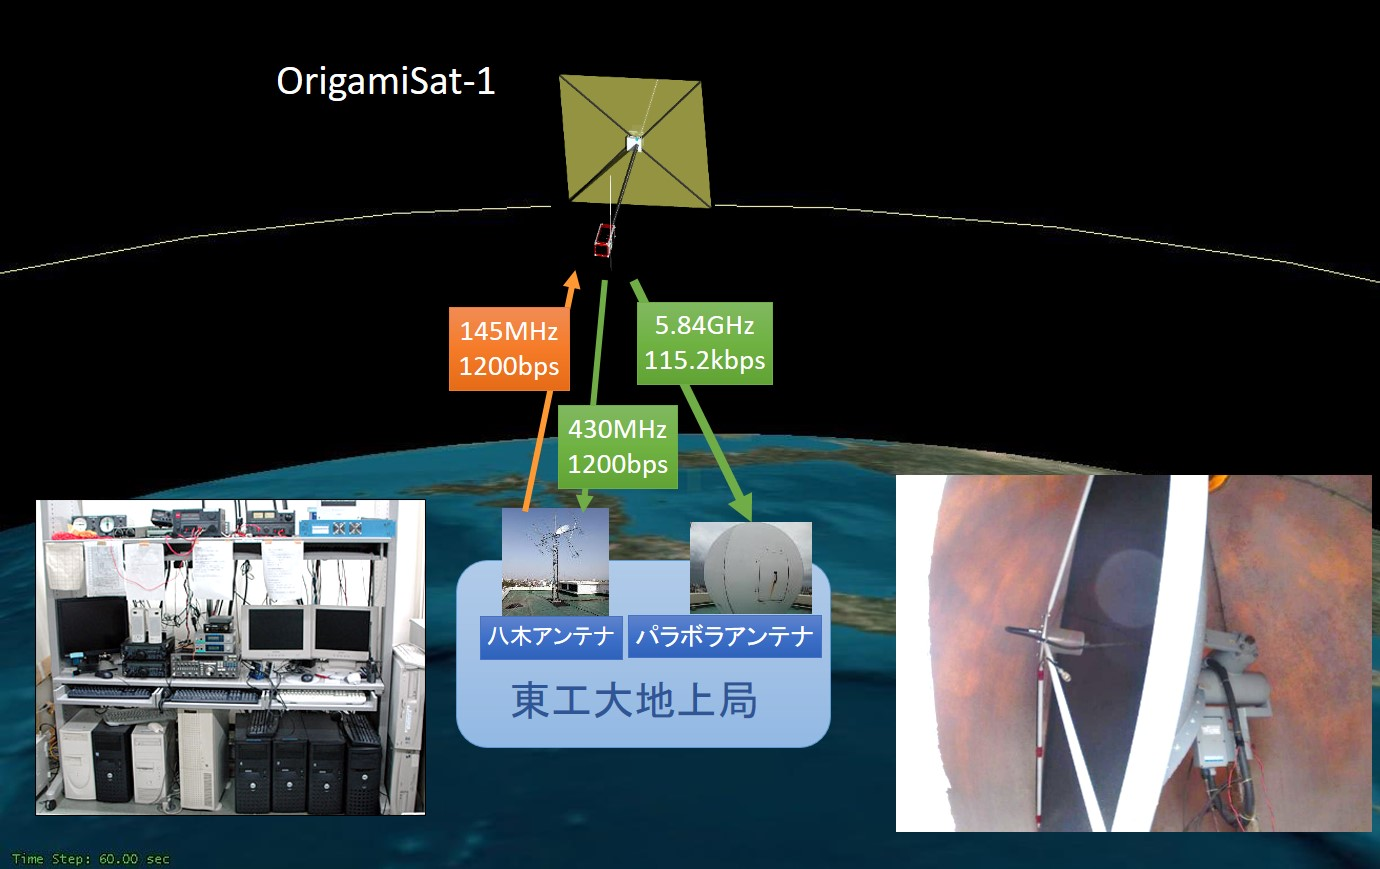
\includegraphics[scale=1]{fig/4/4-2-1.jpg}
%	\caption{図の説明文}
%	\label{fig4-2-1}
%\end{figure}
%
%%表の追加
%\begin{table}[H]
%	\centering
%	\includegraphics[scale=1]{fig/4/t4-2-1.jpg}
%	\caption{表の説明}
%	\label{table4-2-1}
%\end{table}
%********************************

%%%%%%%%%%%%%%%%%%%%%%%%%%%%%%%
\section{放射線試験(寺田(報告書)・池谷・黒崎)}

%%%%%%%%%%%%%%%%%%%%%%%%%%%%%%%
\section{形状計測試験(大野・奥山)}

%%%%%%%%%%%%%%%%%%%%%%%%%%%%%%%
\section{振動試験(加藤・飯島)}

%%%%%%%%%%%%%%%%%%%%%%%%%%%%%%%
\section{衝撃試験(大野)}

%%%%%%%%%%%%%%%%%%%%%%%%%%%%%%%
\section{連続動作試験 EMver(?)}

%%%%%%%%%%%%%%%%%%%%%%%%%%%%%%%
\section{姿勢制御試験(恒光)}

%%%%%%%%%%%%%%%%%%%%%%%%%%%%%%%
\section{通信系 機能試験(大本)}

%%%%%%%%%%%%%%%%%%%%%%%%%%%%%%%
\section{熱真空試験(中村):ベーキングについても言及}

%%%%%%%%%%%%%%%%%%%%%%%%%%%%%%%
\section{表面あらさ計測(大野・奥山)}

%%%%%%%%%%%%%%%%%%%%%%%%%%%%%%%
\section{放出試験(大野・奥山)}